% ICASSP manuscript; to be used with:
%          spconf.sty  - ICASSP/ICIP LaTeX style file, and
%          IEEEbib.bst - IEEE bibliography style file.
% --------------------------------------------------------------------------
\documentclass{article}
\usepackage{spconf,amsmath,booktabs,graphicx,hyperref}
\hypersetup{hidelinks}

% Title.
% ------
\title{CLWE-Prune: Cross-Lingual Worst-Group Excess for Multilingual Text-to-Speech Compression}
%
% Single address.
% ---------------
% \name{Author(s) Name(s)\thanks{Thanks to XYZ agency for funding.}}
\name{
Cuicui Zhu$^{1}$,
Jiawei Zhan$^{1}$,
Xiaoyong Guo$^{1}$,
Hao Huang$^{1,2,3,\dagger}$,
Kai Wang$^{1,2,3,\dagger}$,
Yongchao Wang$^{4}$
}

\address{
$^{1}$\textit{School of Computer Science and Technology, Xinjiang University, Urumqi, China}\\
$^{2}$\textit{Joint International Research Laboratory of Silk Road}\\
\textit{Multilingual Cognitive Computing, Urumqi, China}\\
$^{3}$\textit{Xinjiang Key Laboratory of Multilingual Information Technology, Urumqi, China}\\
$^{4}$\textit{Department of Science and Technology Intelligence, Marketing Service Center of}\\
\textit{State Grid Xinjiang Electric Power Co., Ltd., China}\\
zhu16198@gmail.com,
\{wangkai,huanghao\}@xju.edu.cn,
im\_guoxy@163.com
}


% \address{Author Affiliation(s)}
%
% For example:
% ------------
%\address{School\\
%	Department\\
%	Address}
%
% Two addresses (uncomment and modify for two-address case).
% ----------------------------------------------------------
%\twoauthors
%  {A. Author-one, B. Author-two\sthanks{Thanks to XYZ agency for funding.}}
%	{School A-B\\
%	Department A-B\\
%	Address A-B}
%  {C. Author-three, D. Author-four\sthanks{The fourth author performed the work
%	while at ...}}
%	{School C-D\\
%	Department C-D\\
%	Address C-D}
%

\usepackage{cuted}   % 提供 strip 环境
\usepackage{capt-of} % 提供 \captionof
\usepackage{placeins}
\newcounter{savedtablecounter}


\begin{document}
\ninept
%
\maketitle

\begingroup
\renewcommand{\thefootnote}{\fnsymbol{footnote}}
\footnotetext[2]{Corresponding authors.}
\endgroup
%
\begin{abstract}
English-only layer selection can overlook degradation in other
languages when compressing multilingual text-to-speech (TTS) models.
We propose Cross-Lingual Worst-Group Excess Pruning (CLWE-Prune),
which scores each candidate LLM block by the largest recognition-error
excess caused by its removal from the dense model across English,
Chinese, Japanese, and Korean, and prunes the lowest-scoring blocks.
Recovery fine-tunes pruned models using generated speech-token
sequences screened for text accuracy by offline automatic speech
recognition (ASR). On CosyVoice3, the multilingual \(P_k\)
configurations yield lower four-language average Whisper error than
EN-WER \(P_k\) at all four matched pruning depths. With 400 verified
sequences and 15 updates, recovery reduces Whisper Macro ER by
7.61--10.64\% relative to the corresponding Base checkpoints at
\(P_{12}\), \(P_{15}\), and \(P_{16}\), and lowers SenseVoice Macro ER
at all three depths. With 800 sequences and 40 updates, recovered
\(P_{15}\) retains nine of 24 LLM blocks and has 26.03\% fewer
parameters than Dense-24. Its observed Whisper/SenseVoice Macro ER
is 7.68\%/8.73\%, versus 7.86\%/8.77\% for Dense-24.A separate inference benchmark using a \(P_{15}\) checkpoint shows
RTF decreasing from 0.633 for Dense-24 to 0.375 and first-packet
latency decreasing from 2.600 to 1.572 s.
\end{abstract}
%
\begin{keywords}
Multilingual TTS, Model Compression, Structural Pruning, Cross-Lingual Layer Selection
\end{keywords}
%

\section{Introduction}
\label{sec:intro}

Multilingual text-to-speech (TTS) systems increasingly use a shared
Transformer backbone to synthesize speech across languages
\cite{du2024cosyvoice,du2025cosyvoice3}. Advances in neural TTS have
improved acoustic modeling and waveform generation
\cite{shen2018naturaltts}; prompt-conditioned systems can synthesize
speech for unseen speakers across languages
\cite{casanova2022yourtts,le2023voicebox}; and speech-token models
cast generation as autoregressive sequence prediction
\cite{wang2023neuralcodec,kharitonov2023speak}. This shared backbone,
however, makes streaming inference costly: each autoregressive
decoding step traverses the Transformer blocks in sequence.
Removing entire blocks can shorten this path. Yet a block that
appears dispensable for English may still be crucial for preserving
the linguistic content of speech in languages such as Chinese,
Japanese, and Korean. Aggregate error alone can obscure this risk:
the dense model has different baseline error rates across languages,
while English is evaluated using word error rate (WER) and the other
languages using character error rate (CER). We therefore focus on the
\emph{additional} error caused by pruning within each language,
particularly the largest such increase across languages. Acoustic
quality scores may remain stable even when linguistic content errors
rise.

Structural pruning removes dimensions or layers
\cite{ma2023llmpruner,ashkboos2024slicegpt,men2025shortgpt}. SPADE applies
WER-guided layer selection and distillation to LLM-based TTS
\cite{nguyen2026spade}, but its ranking is English-only and so cannot see
regressions in Chinese, Japanese, or Korean. Averaging scores across languages
is no safety net either: a large drop in one language can hide inside a flat
mean, which is exactly why worst-group evaluation is preferred in robust model
selection \cite{sagawa2020dro}. Pruning multilingual text models can also
shift which language is harmed, as shown for text LLMs under mismatched
calibration \cite{kurz2026limitations}, and ASR-screened self-distillation
has been used to reduce synthesis failures in neural-codec TTS
\cite{asaria2026reliable}. To our knowledge, however, cross-lingual
worst-group block selection combined with ASR-screened student-trajectory
recovery has not been studied for pruned multilingual TTS.

Pruning also changes the student's generation behavior. Standard distillation
trains compact models on teacher information
\cite{hinton2015distilling,kim2016sequence}, but sequences a dense teacher
produces (or that come from recordings) do not match the paths a pruned
student actually walks. On-policy distillation addresses this by learning
from the student's own generated sequences
\cite{agarwal2024onpolicy}, and self-training work shows that generated
supervision must be screened before use \cite{park2020improved}. The risk
here is concrete: a student trajectory that has already mispronounced a
word, if used directly as training signal, teaches the pruned model to
repeat that mistake. For TTS, an offline ASR recognizer can compare the
decoded speech against the requested text and discard trajectories that
fail this content check before they are used. This check runs only in
training; it adds no cost to the deployed synthesizer.

We propose CLWE-Prune, which ranks layers by the worst-group excess error
across four language groups and recovers each pruned model using
ASR-screened student-generated speech-token trajectories, with the acoustic
decoder held fixed. Our contributions are:
\begin{itemize}
\item We propose a cross-lingual layer-selection criterion based on the
largest increase in recognition error relative to the dense model,
improving multilingual content preservation over English-only ranking.

\begin{figure*}[t]
\centering
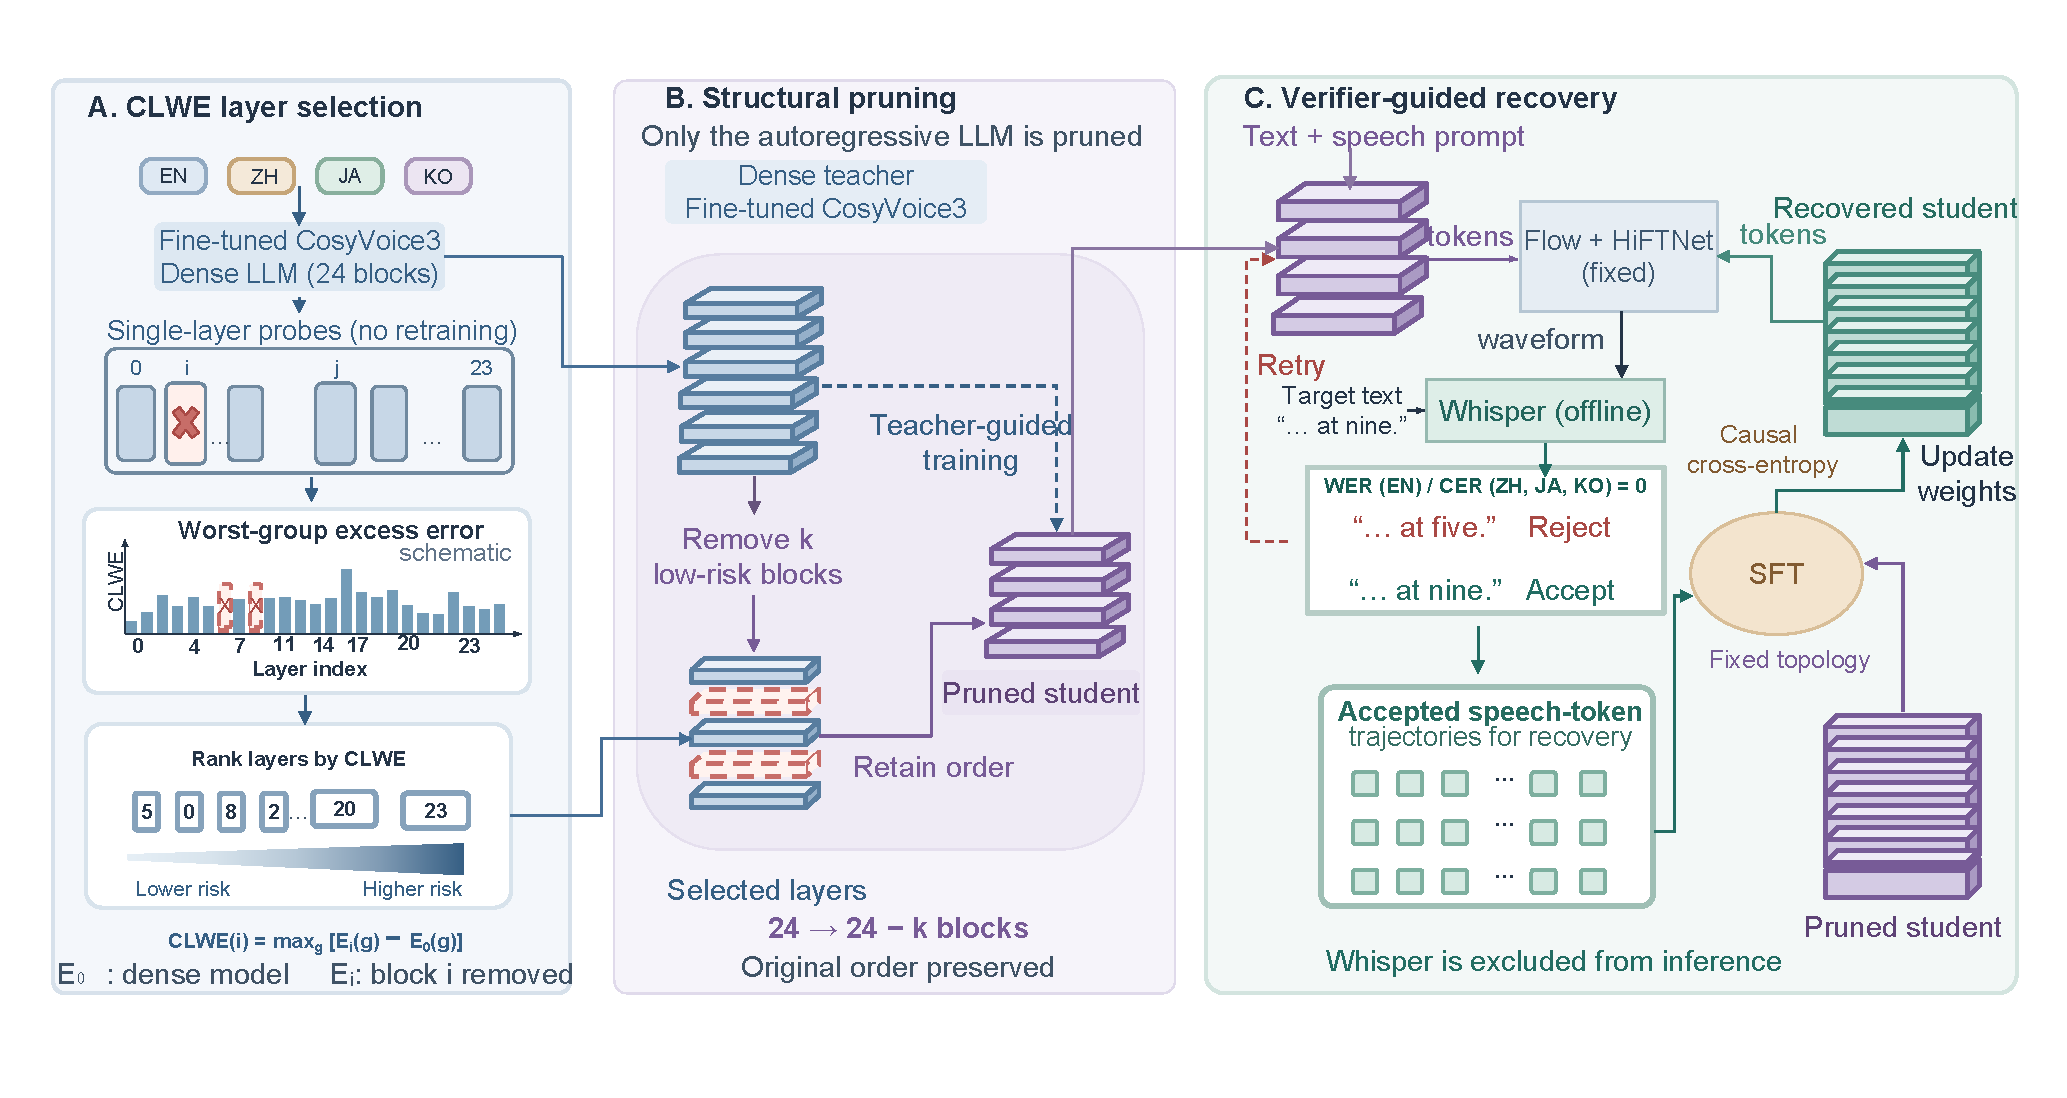
\includegraphics[
width=\textwidth,
keepaspectratio
]{framework.pdf}
\vspace{-2mm}
\caption{Overview of CLWE-Prune. (A) Single-layer removal estimates
cross-lingual worst-group excess risk. (B) Lowest-scoring blocks are
removed and retrained to Base, with the acoustic decoder fixed.
(C) The pruned student is recovered on ASR-screened speech-token
trajectories, keeping the pruning topology fixed.}
\label{fig:framework}
\vspace{-2mm}
\end{figure*}

\setlength{\dbltextfloatsep}{8pt plus 2pt minus 2pt}

\item We introduce verifier-guided recovery using ASR-screened,
student-generated trajectories. This reduces recognition errors without
changing the pruned architecture or acoustic decoder.

\item Our recovered nine-layer model removes $26.03\%$ of the dense
model's parameters while achieving comparable recognition accuracy and
a $1.69\times$ streaming real-time-factor speedup.
\end{itemize}



\section{Method}
\label{sec:method}

Figure~\ref{fig:framework} summarizes three stages: single-layer
risk estimation, physical pruning, and verifier-guided recovery.
We rank CosyVoice3's 24 autoregressive LLM blocks by their
cross-lingual worst-excess error and remove the lowest-risk blocks.
The retained blocks preserve their original order and inherit their
weights from Dense-24. Under the matched-selection protocol, the
pruned LLM undergoes continuation training guided by a frozen
Dense-24 teacher; the checkpoint with the lowest validation loss
becomes the Base model. Recovery then fine-tunes this Base model on
ASR-screened, student-generated speech-token trajectories. The
teacher used to construct Base is distinct from the Dense-Teacher
recovery control, which supplies recovery targets. The flow-matching
acoustic model and HiFTNet vocoder remain unchanged throughout.

\subsection{CLWE-Based Layer Selection}
\label{sec:clwe_selection}

As shown in Fig.~\ref{fig:framework}(A), we estimate single-block
removal risk on a multilingual layer-selection dataset. We group
samples by language, with one group per language. Thus,

$\mathcal{G}=\{g_{\mathrm{EN}},g_{\mathrm{ZH}},
g_{\mathrm{JA}},g_{\mathrm{KO}}\}$.

To probe block $i$, we remove only that block from Dense-24 and
evaluate the remaining model without retraining. All single-block
probes use the same inference and scoring procedure. Let $E_i(g)$
and $E_0(g)$ denote the recognition errors of the probe and
Dense-24, respectively, on language group $g$.

Following SPADE's WER-based layer-importance approach
\cite{nguyen2026spade}, the English-only baseline ranks block $i$ by
$R_i^{\mathrm{EN}}=E_i(g_{\mathrm{EN}})$. Subtracting the constant
$E_0(g_{\mathrm{EN}})$ from every English score would leave this
ranking unchanged. This baseline compares layer-selection criteria;
it does not reproduce the full SPADE training pipeline.

CLWE instead measures the additional error caused by removing each
block within each language:
\begingroup
\setlength{\abovedisplayskip}{3pt}
\setlength{\abovedisplayshortskip}{3pt}
\setlength{\belowdisplayskip}{3pt}
\setlength{\belowdisplayshortskip}{3pt}
\begin{equation}
\begin{aligned}
\Delta_i(g) &= E_i(g)-E_0(g),\\
R_i^{\mathrm{CLWE}}
&= \max_{g\in\mathcal{G}}\Delta_i(g).
\end{aligned}
\label{eq:clwe_risk}
\end{equation}
\endgroup
Subtracting $E_0(g)$ accounts for each language's Dense-24 baseline,
while the maximum makes the largest observed error increase determine
the block's risk. This subtraction does not make English WER
statistically equivalent to the other languages' CER. A lower
$R_i^{\mathrm{CLWE}}$ indicates a safer block to remove.

We rank blocks in ascending order of risk, breaking ties by their
original indices. For a pruning budget of $k$, we physically remove
the first $k$ blocks in this ranking, as shown in
Fig.~\ref{fig:framework}(B). The ranking is computed once and reused
across pruning depths, so the removal sets are nested and the
retained blocks keep their original order. Single-block probes do not
capture interactions among jointly removed blocks; consequently,
their ranking is a selection heuristic, not a bound on the final
pruned model's error.

\subsection{Verifier-Guided Student-Trajectory Recovery}
\label{sec:verifier_recovery}

As shown in Fig.~\ref{fig:framework}(C), each pruned Base model
generates speech-token trajectories
$\mathbf{z}=(z_1,\ldots,z_T)$ conditioned on text $x$ and prompt $c$.
Generation uses temperature 1.0, \texttt{top\_p}=0.8, and
\texttt{top\_k}=25. The fixed flow-matching acoustic model and
HiFTNet vocoder decode the tokens into speech. After
language-specific text normalization, Whisper evaluates content
using WER for English and CER for Chinese, Japanese, and Korean.

Zero-error candidates are prioritized. When an input has no
acceptable candidate, we generate additional candidates or draw
from a shared reserve text pool. Among candidates passing the
content check, speaker similarity, UTMOS, and duration ratio guide
selection; these quality measures do not replace the ASR criterion.
Candidate generation and screening are performed offline.

Each pruned student Base first generates 400 speech-token
trajectories, from which we select recovery targets using the
verifier. We fine-tune the student on these targets and report
its step-15 checkpoint as SFT400/15. This checkpoint then
generates a second set of 400 verifier-screened targets.

For SFT800/40, we reinitialize the student from its original
pruned Base checkpoint and fine-tune it on both sets of targets.
We report the resulting step-40 checkpoint. Thus, SFT400/15
generates the second target set but is not the initialization
for SFT800/40. In the P12 Base-generated control, both sets
of targets are generated by the original P12 Base, while the
final model is trained from that same Base.

Let $\mathcal{D}_{\mathrm{rec}}$ contain the accepted trajectories.
For sequence $j$ in a minibatch $\mathcal B$, set
$\tilde z_{j,t}=z_{j,t}$ for $t\leq T_j$ and
$\tilde z_{j,T_j+1}=\mathrm{EOS}$. With
$h_{j,t}=(x_j,c_j,\tilde z_{j,<t})$, we optimize
\begin{equation}
\mathcal{L}_{\mathrm{rec}}
=-\frac{1}{N_{\mathcal B}}\sum_{j,t}
\log p_{\theta_{\mathrm P}}
(\tilde z_{j,t}\mid h_{j,t}).
\label{eq:recovery_loss}
\end{equation}
Here $\sum_{j,t}$ ranges over $j\in\mathcal B$ and
$t=1,\ldots,T_j+1$, while
$N_{\mathcal B}=\sum_{j\in\mathcal B}(T_j+1)$ counts valid targets,
excluding masked text and padding positions. The parameters
$\theta_{\mathrm P}$ belong to the pruned LLM. Recovery uses a
learning rate of $3\times10^{-6}$ and mixed precision. Teacher
forcing trains the LLM to predict the accepted sequences; Whisper
provides no training gradients.



\subsection{Experimental Setup}
\label{sec:setup}

\noindent\textbf{Data.}
The calibration set uses 400 utterances per language--corpus group from LibriTTS
(English) \cite{zen2019libritts}, AISHELL-3 (Chinese)
\cite{shi2021aishell3}, and Emilia (Japanese and Korean)
\cite{he2025emilia}. The \texttt{strict1200} test set has 300 utterances
per language. Models share test texts and prompts but generate separate
waveforms. Recovery uses 100 or 200 targets per language for
SFT400/15 or SFT800/40.

\noindent\textbf{Models and training configurations.}
Dense-24 is the unpruned 24-block model. Removing \(k\) LLM blocks
leaves \(24-k\) blocks. Multilingual configurations selected by CLWE
at this depth are labeled \(P_k\), and the English-only pruning
baseline is labeled EN-WER \(P_k\).
Table~\ref{tab:criterion_comparison} compares both at
\(k\in\{6,8,10,12\}\). Table~\ref{tab:high_compression} extends the
multilingual sweep to \(P_{13}\)--\(P_{17}\). Its separate inference
benchmark reports Dense-24, \(P_{12}\), \(P_{15}\), and \(P_{16}\).

Table~\ref{tab:recovery_results} compares recovery from \(P_{12}\),
\(P_{15}\), and \(P_{16}\) Base checkpoints, which are separate from
the Table~\ref{tab:high_compression} sweep. Verifier-SFT
is evaluated at both 400/15 and 800/40 for all three depths. At
\(P_{12}\), additional controls include Base-Generated-SFT800/40,
Selected-Original400/15 using original-recording tokens, and
Random-Candidate400/15 using unverified student targets with
separately assigned same-language prompts. Dense-Teacher-SFT400/15
uses verified dense-model targets at all three depths. Dense-24
Teacher is the unpruned reference.

\noindent\textbf{Evaluation metrics.}
Content accuracy is evaluated using Whisper large-v3
\cite{radford2023whisper} and SenseVoiceSmall
\cite{an2024funaudiollm}. WER is used for English, while CER is used for Chinese,
Japanese, and Korean. We report macro-averaged error rate (Macro ER),
computed as the mean of the four language-level error rates.
Table~\ref{tab:recovery_results} averages decoding seeds 1986--1988
per fixed checkpoint.
For a model
evaluated alongside Dense-24, the test worst-group excess is
$\max_g[E_{\rm model}(g)-E_{\rm Dense}(g)]$.

We report UTMOS predicted quality \cite{saeki2022utmos} and
mel-cepstral distortion (MCD) in the recovery comparison. The
high-compression sweep also reports CAM++ speaker embedding cosine
similarity (SECS) \cite{wang2023campp}. MCD uses 24-kHz WORLD
24-order mel cepstra (excluding $c_0$) aligned with fastDTW.
Higher UTMOS/SECS and lower MCD are preferred. UTMOS also ranks candidates; these automatic scores do not establish perceived naturalness.
A separate architecture benchmark measures
streaming real-time factor (RTF), first-packet latency, and peak allocated CUDA memory.

\par\smallskip
\noindent\begin{minipage}{\columnwidth}
\centering
\captionof{table}{English-WER versus multilingual CLWE layer
selection. Bold marks values where \(P_k\) outperforms EN-WER \(P_k\)
at the same depth.}
\label{tab:criterion_comparison}
\small
\setlength{\tabcolsep}{1.0pt}
\renewcommand{\arraystretch}{1.05}
\begin{tabular}{lcccc}
\toprule
\textbf{Model} &
\textbf{Macro$\downarrow$} &
\textbf{EN/ZH$\downarrow$} &
\textbf{JA/KO$\downarrow$} &
\textbf{UTMOS$\uparrow$/MCD$\downarrow$} \\
\midrule
EN-WER P6 & 7.92 & 2.16/12.17 & 12.12/5.26 & 3.47/8.32 \\
P6 & \textbf{7.67} & 2.75/\textbf{11.67} & \textbf{11.92}/\textbf{4.34} & \textbf{3.48}/\textbf{8.28} \\
EN-WER P8 & 7.91 & 2.23/12.67 & 11.93/4.81 & 3.47/8.32 \\
P8 & \textbf{7.65} & \textbf{2.04}/\textbf{12.01} & 12.16/\textbf{4.37} & \textbf{3.48}/\textbf{8.26} \\
EN-WER P10 & 8.47 & 2.81/11.97 & 13.85/5.27 & 3.48/8.27 \\
P10 & \textbf{7.78} & \textbf{2.53}/12.28 & \textbf{11.45}/\textbf{4.88} & 3.47/8.29 \\
EN-WER P12 & 8.97 & 2.64/12.10 & 16.25/4.90 & 3.49/8.31 \\
P12 & \textbf{8.09} & \textbf{2.42}/12.38 & \textbf{12.51}/5.04 & 3.48/8.32 \\
\bottomrule
\end{tabular}%
\end{minipage}\par\smallskip

\subsection{Results and Analysis}
\label{sec:results}

\par\smallskip
\noindent\begin{minipage}{\columnwidth}
\centering
\captionof{table}{High-compression quality sweep and separate architecture
inference benchmark. L denotes retained blocks. Macro ER is Whisper Macro ER.}
\label{tab:high_compression}

\setlength{\tabcolsep}{2.5pt}
\renewcommand{\arraystretch}{1.05}
\begin{tabular}{@{}lccccc@{}}
\toprule
\textbf{Model} & \textbf{Layers} & \textbf{Macro ER$\downarrow$} &
\textbf{UTMOS$\uparrow$} & \textbf{SECS$\uparrow$} &
\textbf{MCD$\downarrow$} \\
\midrule
P13 & 11 & 8.36  & 3.48 & 0.80 & 8.31 \\
P14 & 10 & 8.65  & 3.48 & 0.80 & 8.36 \\
P15 &  9 & 8.75  & 3.48 & 0.80 & 8.35 \\
P16 &  8 & 11.31 & 3.47 & 0.80 & 8.40 \\
P17 &  7 & 13.17 & 3.48 & 0.80 & 8.46 \\
\bottomrule
\end{tabular}\par\vspace{0.6mm}

\begin{tabular}{@{}lcccc@{}}
\toprule
\textbf{Model} &
\shortstack{\textbf{Params}\\\textbf{(M)$\downarrow$}} &
\textbf{RTF$\downarrow$} &
\shortstack{\textbf{First pkt.}\\\textbf{(s)$\downarrow$}} &
\shortstack{\textbf{Peak CUDA}\\\textbf{(MiB)$\downarrow$}} \\
\midrule
Dense-24 & 859.19 & 0.633 & 2.600 & 3382 \\
P12      & 680.24 & 0.434 & 1.779 & 2697 \\
P15      & 635.50 & 0.375 & 1.572 & 2530 \\
P16      & 620.59 & 0.377 & 1.535 & 2468 \\
\bottomrule
\end{tabular}\par
\end{minipage}\par\smallskip

% Queue the wide recovery table early enough for a preceding page-top pass.
% Reserve Table 3 while preserving the numbering of the two in-text tables.
\begin{table*}[!t]
\centering
\caption{Recovery performance on \texttt{strict1200}.
W and SV denote Whisper large-v3 and SenseVoiceSmall.
Bold marks the best value within each pruning depth;
Dense-24 Teacher is the unpruned reference.}
\label{tab:recovery_results}
\small
\setlength{\tabcolsep}{3pt}
\renewcommand{\arraystretch}{1.05}
\begin{tabular}{lcccccccc}
\toprule
\textbf{Recovery Model} & \textbf{W-Macro$\downarrow$} &
\textbf{SV-Macro$\downarrow$} &
\textbf{EN W/SV} & \textbf{ZH W/SV} & \textbf{JA W/SV} &
\textbf{KO W/SV} & \textbf{UTMOS$\uparrow$} & \textbf{MCD$\downarrow$} \\
\midrule
P12 (Base) & 8.15 & 9.23 &
2.64/4.11 & 12.36/10.86 & 12.36/14.19 & 5.23/7.76 & 3.4884 & 8.3143 \\
P12 + Verifier-SFT400/15 & 7.53 & 8.40 &
2.61/3.75 & 11.79/10.56 & 11.16/12.41 & 4.58/6.87 & 3.5241 & 8.2449 \\
P12 + Verifier-SFT800/40 & \textbf{7.24} & \textbf{8.32} &
\textbf{2.36}/\textbf{3.68} & 11.51/10.45 & \textbf{10.76}/\textbf{12.39} & \textbf{4.35}/6.74 & \textbf{3.5496} & 8.2541 \\
P12 + Base-Generated-SFT800/40 & 7.62 & 8.33 &
2.55/3.88 & 12.01/10.39 & 11.51/12.40 & 4.39/\textbf{6.64} & 3.5411 & 8.2609 \\
P12 + Selected-Original400/15 & 8.28 & 9.34 &
2.59/4.12 & 12.25/10.71 & 12.50/14.50 & 5.77/8.05 & 3.4746 & 8.2967 \\
P12 + Random-Candidate400/15 & 7.62 & 8.53 &
2.54/3.98 & 12.20/10.67 & 11.33/12.59 & 4.41/6.89 & 3.5133 & \textbf{8.2388} \\
P12 + Dense-Teacher-SFT400/15 & 7.68 & 8.57 &
2.61/4.14 & \textbf{7.16}/\textbf{5.32} & 15.53/16.83 & 5.41/7.99 & 3.5404 & 8.3762 \\
\addlinespace
P15 (Base) & 8.91 & 9.73 &
3.00/4.40 & 12.17/10.88 & 13.54/15.07 & 6.94/8.56 & 3.4788 & 8.3662 \\
P15 + Verifier-SFT400/15 & 8.00 & \textbf{8.59} &
2.78/\textbf{4.02} & 12.27/10.78 & 12.39/12.48 & \textbf{4.54}/\textbf{7.08} & 3.5280 & \textbf{8.2871} \\
P15 + Verifier-SFT800/40 & \textbf{7.68} & 8.73 &
\textbf{2.72}/4.24 & 12.09/10.81 & \textbf{11.09}/\textbf{12.44} & 4.83/7.43 & \textbf{3.5543} & 8.2912 \\
P15 + Dense-Teacher-SFT400/15 & 8.82 & 9.44 &
2.93/4.55 & \textbf{7.74}/\textbf{5.81} & 18.72/18.65 & 5.90/8.76 & 3.5282 & 8.4419 \\
\addlinespace
P16 (Base) & 9.87 & 10.80 &
3.65/5.30 & 12.69/11.09 & 15.58/17.13 & 7.57/9.69 & 3.4721 & 8.4053 \\
P16 + Verifier-SFT400/15 & 8.82 & 9.50 &
3.38/\textbf{4.54} & 12.35/11.02 & 14.02/14.07 & \textbf{5.54}/8.35 & 3.5345 & 8.3495 \\
P16 + Verifier-SFT800/40 & \textbf{8.32} & \textbf{9.27} &
\textbf{3.21}/4.78 & 12.36/11.12 & \textbf{12.09}/\textbf{13.20} & 5.62/\textbf{7.96} & \textbf{3.5688} & \textbf{8.3476} \\
P16 + Dense-Teacher-SFT400/15 & 10.16 & 10.80 &
3.78/5.28 & \textbf{8.01}/\textbf{6.16} & 21.75/22.44 & 7.08/9.31 & 3.5249 & 8.4836 \\
\addlinespace
Dense-24 Teacher & 7.86 & 8.77 &
2.13/3.39 & 12.21/10.67 & 13.72/14.48 & 3.39/6.52 & 3.4724 & 8.3113 \\
\bottomrule
\end{tabular}
\end{table*}

\setlength{\dbltextfloatsep}{8pt plus 2pt minus 2pt}

Table~\ref{tab:criterion_comparison} compares layer rankings at
matched depths. The multilingual \(P_k\) models lower Whisper Macro ER
by 0.25, 0.26, 0.69, and 0.88 points at P6, P8, P10, and P12.
The largest reported language error also falls by 0.25, 0.51, 1.57,
and 3.74 points, respectively. This descriptive maximum mixes English
WER with the other languages' CER. P12 Japanese CER (16.25\% to
12.51\%) shows the non-English regression missed by English-only
ranking. P10 Chinese CER rises by 0.31 points, so gains are not
uniform. Mean-Excess and Max-Raw checkpoints were not evaluated, so
this comparison does not isolate the maximum operation or
Dense-baseline subtraction. The matched comparison ends at P12.

Table~\ref{tab:high_compression} reports available multilingual
\(P_k\) configurations, not a controlled depth-only ablation.
Whisper Macro ER rises from 8.36\% at P13 to 8.75\% at P15 and
11.31\% at P16, while UTMOS and SECS barely change. This motivates
testing recovery at \(P_{15}\) and \(P_{16}\). In the separate
architecture benchmark, RTF falls from 0.633 for Dense-24 to 0.375
for \(P_{15}\) (1.69$\times$). First-packet latency falls from 2.600
to 1.572 s. These efficiency checkpoints are distinct from the
quality and recovery checkpoints. Peak allocated CUDA memory falls
from 3382 to 2530 MiB. The \(P_{16}\) architecture has a slightly
lower first-packet latency (1.535 s) but no further RTF gain (0.377).
The measured quality and efficiency trends favor \(P_{15}\) among
these configurations.

Relative to their respective Base models in
Table~\ref{tab:recovery_results}, Verifier-SFT400/15 reduces
Whisper/SenseVoice Macro ER by 0.62/0.83, 0.91/1.14, and 1.05/1.30
points at P12, P15, and P16, respectively. UTMOS increases and MCD
decreases at each depth without changing parameter counts. SenseVoice
does not select targets, so its improvement supports a content gain
beyond the Whisper screening metric. Among 24 per-language ASR values
(three depths, four languages, two recognizers), 23 decrease. The sole
exception is P15 Chinese Whisper CER (12.17\% to 12.27\%). This breadth
shows that the macro gains are not driven by one language. UTMOS also
ranks accepted targets.

SFT800/40 further improves both ASR measures at P12 and P16. At P15,
Whisper improves from 8.00 to 7.68 but SenseVoice rises from 8.59 to
8.73. Relative to their own Base checkpoints, the P15 and P16
SFT800/40 models reduce Whisper/SenseVoice Macro ER by
1.23/1.00 and 1.55/1.53 points, respectively.
At P15, UTMOS increases from 3.4788 to 3.5543 and
MCD decreases from 8.3662 to 8.2912. These automatic acoustic scores
move with the recognition gains, although UTMOS is also used to rank
accepted recovery candidates. The recovered \(P_{15}\) model has
635.50M total parameters, versus 859.19M for Dense-24, and observed
Macro ER of 7.68/8.73 versus 7.86/8.77. Its worst-group Whisper
excess over Dense-24 is still 1.44 points in Korean (4.83 versus
3.39). English WER is also 0.59 points higher. Thus, the lower macro
average does not imply uniform language-level preservation.

At P12, Selected-Original is slightly worse than Base (8.28/9.34
versus 8.15/9.23), while Random-Candidate reaches 7.62/8.53 and
verified student recovery reaches 7.53/8.40. Student-generated targets
give the larger observed gain, consistent with the on-policy rationale
\cite{agarwal2024onpolicy}. Different prompts prevent assigning the
smaller verified--random gap solely to ASR screening. With 800 targets,
mixed Base/auxiliary generation reaches 7.24/8.32 versus 7.62/8.33
when Base generates all targets, with separate training runs.
Dense-Teacher at P15 lowers Chinese Whisper CER from 12.17\% to 7.74\%
but raises Japanese CER from 13.54\% to 18.72\%. At the same 400-target/15-update setting, verified student targets
yield lower Whisper/SenseVoice Macro ER than Dense-Teacher targets by
0.15/0.17, 0.82/0.85, and 1.34/1.30 points at P12, P15, and P16. The Japanese
Whisper CER gap is especially large at P15 (12.39\% versus 18.72\%)
and P16 (14.02\% versus 21.75\%), whereas the teacher targets improve
Chinese. Thus the lower macro errors do not merely reflect a single
favorable language.
\section{Conclusion}
\label{sec:conclusion}

We presented CLWE-Prune, which ranks LLM blocks by worst-group
recognition-error excess across four languages and recovers pruned
models using ASR-screened student trajectories, with the acoustic
decoder held fixed. At all four matched depths, the multilingual
\(P_k\) configurations have lower Whisper Macro ER than EN-WER
\(P_k\); at \(P_{12}\), Japanese CER is 12.51\% versus 16.25\% for
EN-WER \(P_{12}\). With Verifier-SFT400/15, 23 of 24 per-language
ASR values improve relative to the corresponding Base checkpoints
across \(P_{12}\), \(P_{15}\), and \(P_{16}\). Recovered \(P_{15}\)
with SFT800/40 has 26.03\% fewer parameters than Dense-24 and
slightly lower observed Whisper/SenseVoice Macro ER. Relative to
the corresponding Base checkpoints, dense-teacher targets reduce
Chinese errors but increase Japanese errors at all three depths;
under the matched 400/15 budget, verified student targets yield
lower macro errors. Language-level gaps remain, notably in English
and Korean. Joint selection and recovery, broader language coverage,
and human evaluation are left for future work.

\section{Compliance with Ethical Standards}
This study used existing publicly available speech corpora and
involved no new data collection or interaction with human
participants. No additional ethical approval was required.

% Before submission, add an Acknowledgment section here after the
% authors confirm funding, competing interests, and generative-AI use.

% uncomment the preceding line ``\centerline...'' and replace ``imageX.ps''
% with a suitable PostScript file name.
% -------------------------------------------------------------------------




% References should be produced using the bibtex program from suitable
% BiBTeX files (here: strings, refs, manuals). The IEEEbib.bst bibliography
% style file from IEEE produces unsorted bibliography list.
% -------------------------------------------------------------------------
\bibliographystyle{IEEEbib}
\begingroup\small
\setlength{\itemsep}{0pt}
\bibliography{refs}
\endgroup

\end{document}


